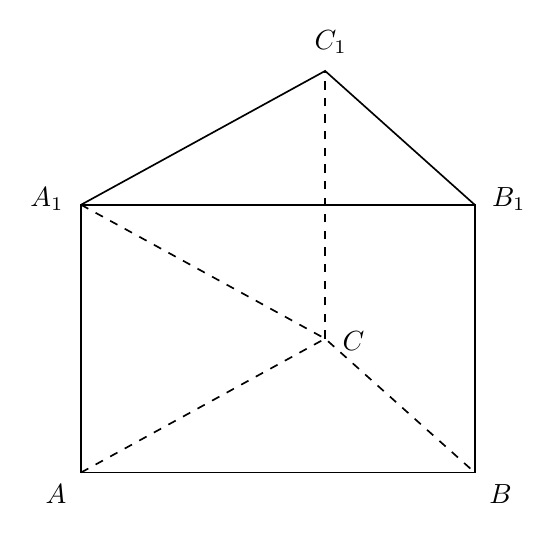
\begin{tikzpicture}[x=1cm,y=1cm,line width=.6pt,font=\normalsize]
% Triangular prism ABC-A1B1C1, front view: ABB1A1 rectangle, C inside, C1 top
\coordinate (A) at (0,0);
\coordinate (B) at (5,0);
\coordinate (A1) at (0,3.4);
\coordinate (B1) at (5,3.4);
\coordinate (C) at (3.1,1.7);
\coordinate (C1) at (3.1000000000,5.1000000000);
% solid outline
\draw (A) -- (B) -- (B1) -- (A1) -- cycle;

\draw (A1) -- (C1) -- (B1);
% hidden dashed
\draw[dashed] (A) -- (C) -- (B);
\draw[dashed] (A1) -- (C);
\draw[dashed] (C) -- (C1);
% labels with clearance
\node[anchor=north east,inner sep=1pt] at ([xshift=-4pt,yshift=-3pt]A) {$A$};
\node[anchor=north west,inner sep=1pt] at ([xshift=4pt,yshift=-3pt]B) {$B$};
\node[anchor=east,inner sep=1pt] at ([xshift=-5pt,yshift=2pt]A1) {$A_{1}$};
\node[anchor=west,inner sep=1pt] at ([xshift=5pt,yshift=2pt]B1) {$B_{1}$};
\node[anchor=west,inner sep=1pt] at ([xshift=5pt,yshift=-1pt]C) {$C$};
\node[anchor=south,inner sep=1pt] at ([xshift=2pt,yshift=5pt]C1) {$C_{1}$};
\end{tikzpicture}
